\documentclass{standalone}
\usepackage{tikz}
\usepackage{animate}
\usepackage{amsmath}
\usepackage{ifthen}
\usetikzlibrary {matrix}
\usepackage{tikzlings}
\usepackage{tikzlings-penguins}

\begin{document}
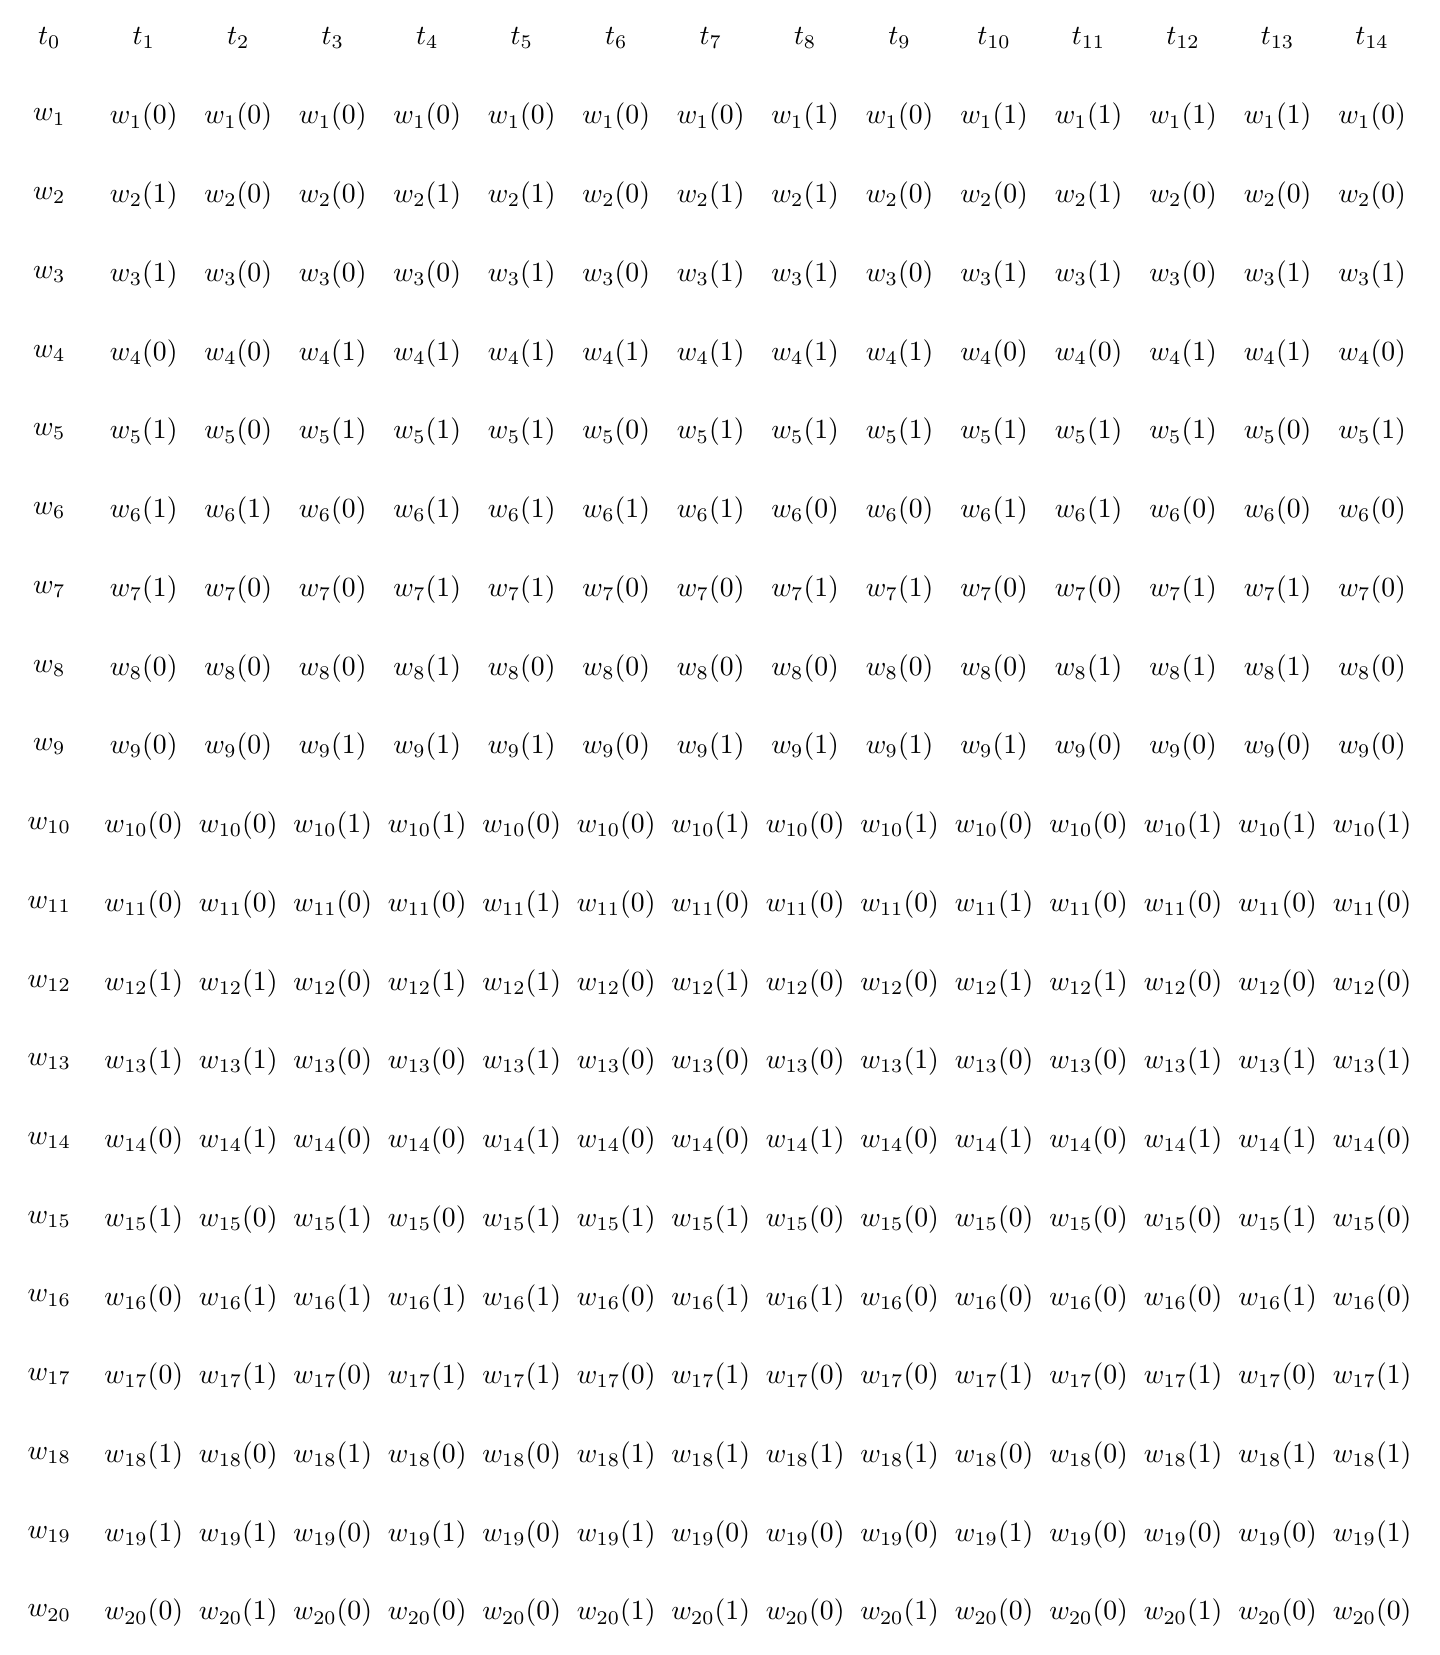
\begin{tikzpicture}[inner sep =0mm,>=latex,thick,x=1.2cm,y=1cm]
  \begin{scope} 
    \xdef\ww{20} 
    \xdef\wwm{ 19}
    \xdef\stagem {13} 
    \xdef\stage {14} 
    \xdef\stagep{15} 


    \foreach \i in {\stagep,\stage,...,1} {
      \pgfmathparse { int(\stagep-\i)}
      \xdef\tt { \pgfmathresult} 
      \node  (t_\i) at ( -\i,0)  { $t_{\tt}$};
    }
    \foreach \i in { \stage,\stagem,...,1} {
      \foreach \j in { 1,2,...,\ww} {
        \pgfmathparse{random(0,1)}
        \xdef\label{\pgfmathresult}
        \node[]   (a_\i\j)  at (-\i,-\j )  { $w_{\j}(\label)$};
     }
    }
    \foreach \j in { 1,2,...,\ww} {
      \node  (w_\j) at ( -\stagep,-\j)  { $w_{\j}$};
    }
  \end{scope}

\end{tikzpicture}


\end{document}
